\chapter{Making Solid Bodies}

\label{sec:making_solid_bodies}

In Chapter \ref{sec:planar-pulleys}, we used a 3D sketch to make three lines and
two circles, a task easily accomplished with a 2D sketch. We did this for two
reasons. First, this is a nice introduction to using 3D sketches. Second, this
added bit of complication will allow us to reconfigure our pulleys and cables
out of plane without major Feature Tree rework.

In Chapter \ref{sec:making_solid_bodies}, we're going to turn this sketch into
solid bodies by the following process:

\begin{enumerate}
  \item{} Add a second \relation{3D Sketch} (egads!) that contains just the cable path.
\item{} \relation{Sweep} a circular cable profile along that path.
\item{} \relation{Revolve} a pulley about the pulley axis.
\item{} \kode{Copy} \cadsymbol{move-copy} that pulley to the location of the second pulley (optional).
\item{} \relation{Mirror} each half-pulley into a full pulley.
\end{enumerate}

The labels we'll use for our solid bodies are shown in
Figure~\ref{fig:labeled-bodies}.

\begin{figure}[H]
\begin{center}
  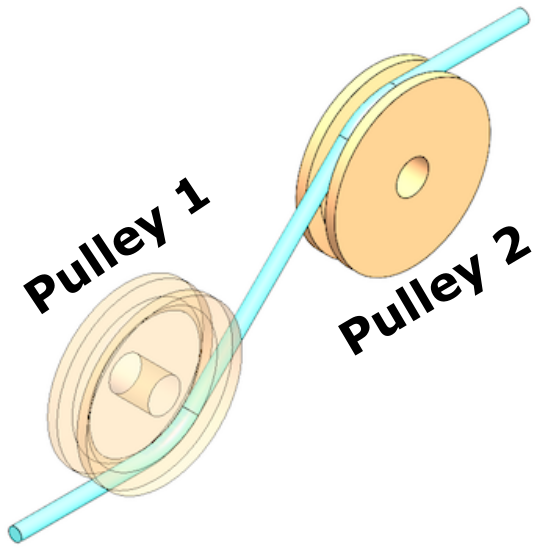
\includegraphics[height=3in]{images/figures/completed-planar-labeled.png}
\end{center}
\caption{
\label{fig:labeled-bodies}}
\end{figure}

\section{Another 3D Sketch}

\label{sec:second-3d-sketch}

My preferred style is to transfer all of the lines that make up the cable path
to a separate 3D sketch. I've found this addition makes the part file easier to
work with and more, rather than less, stable.

Add a \kode{3D Sketch} as in Section \ref{sec:making_line_1}. Next, \kode{Convert
Entities} 
\includegraphics{images/symbols/convert-entities.png} and select \emph{Lines 1, 2, \& 3}, and \emph{Circles 1 \& 2}. This will bring these five
entities to the current 3D sketch and give them all \relation{On-Edge} relations.

Finally, we must trim the circles to make them into arcs. Select the \relation{Trim}
tool, and change the settings to ``Trim to closest''. Click on the segment
of \emph{Circle~1} where the cable won't run, and this will remove it. Do the same for
\emph{Circle~2}. You should be left with the curve shown in Figure~\ref{fig:second-3d-sketch}. Close this sketch
\cadsymbol{close-sketch}.

\begin{figure}[H]
\begin{center}
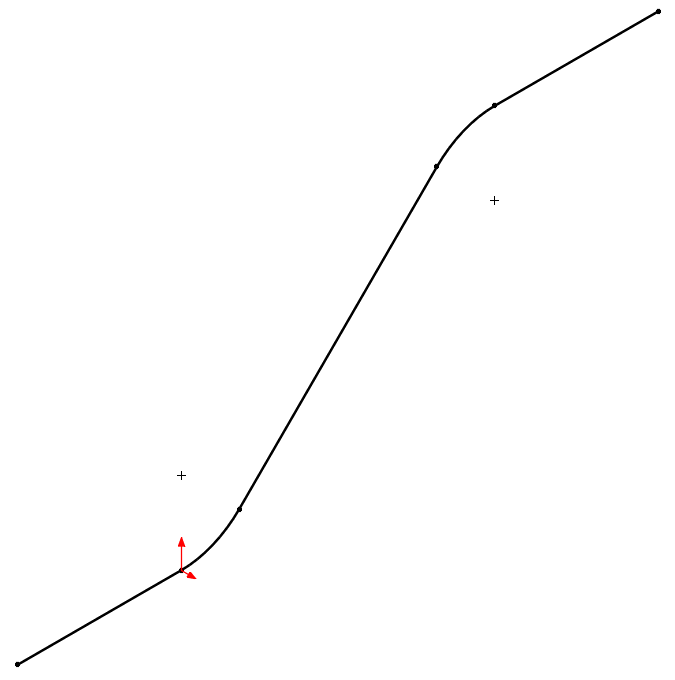
\includegraphics[height=3in]{images/figures/second-3d-sketch.png}
\end{center}
\caption{The results of our second 3D sketch. This curve will be the path in our
\kode{Swept Boss/Base}.
\label{fig:second-3d-sketch}}

\end{figure}

\subsubsection{Why another 3D sketch?}

I separate the geometry of my cable path (from Chapter~\ref{sec:planar-pulleys})
from the path used in the sweep (from Section~\ref{sec:second-3d-sketch}) for
these reasons:

\begin{enumerate}
\item{} This prevents my geometry sketch from being absorbed into the Sweep feature,
making it easier to find in the Feature Tree later.
\item{} This allows my geometry sketch to contain more than just lines and arcs.
Sweep paths (Section~\ref{sec:cable_sweep}) require a single continuous
non-overlapping curve, a rather strict requirement for a geometry sketch.
\end{enumerate}

\subsubsection{Section Recap}

\begin{enumerate}
\item{} Create a new \relation{3D Sketch}.
\item{} \relation{Convert Entities} to bring the three lines and two circles to this 3D
sketch.
\item{} \relation{Trim} the circles into arcs to make a smooth curve, shown in Figure~\ref{fig:second-3d-sketch}.
\end{enumerate}

\begin{aside}
\label{aside:3d_sketch_warning}
\heading{A Word of Warning}

When I learned 3D sketches, I applied them to all sorts of designs. Why make 3
sketchs when I can could put all my entites into a single 3D sketch? Like
elephant guns or Lagrangian mechanics, 3D sketches are useful in a few specific
instances but are otherwise unwieldy and
inefficient. They're mostly useful when the plane of a feature is unknown and is
determined by sketch geometry. Nothing we've done in the tutorial thus far
requires a 3D sketch.

\end{aside}

\section{Make the Cable with a Sweep}

\label{sec:cable_sweep}
To create our cable, we will use a \kode{Swept Boss/Base} \cadsymbol{Sweep}, which seems a rather
lengthy name for a \relation{Sweep}. We haven't defined our cable cross-section yet, so
that's Phase 1\footnote{Phase 3: Profit}.

Sketch a circle on the Front Plane which, if all has gone to plan, is normal to
our cable path. Dimension this circle to 0.1''. You should end up
with Figure~\ref{fig:sweep-cross-section}.

\begin{figure}[H]
\begin{center}
  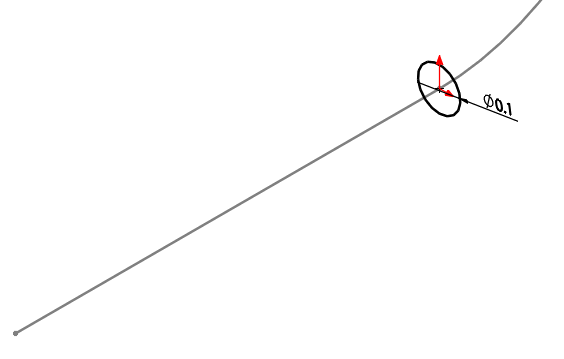
\includegraphics[height=3in]{images/figures/sweep-cross-section.png}
\end{center}
\caption{Sweep path and cross-section.
\label{fig:sweep-cross-section}}

\end{figure}

Add a \relation{Sweep} feature. Select \emph{3D Sketch 2} as the path, and \emph{Sketch 1} as the
cross-section. Turn on the ``Show preview''. Select ``Bidirectional'' 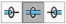
\includegraphics{images/symbols/bidirectional-sweep.png} to make the sweep extend to
both ends of the path. My Sweep property manager dialog is shown in Figure~\ref{fig:sweep-feature-tree}. Close this feature, and you should end up with a
lovely, sweeping curve as in Figure~\ref{fig:completed-cable-sweep}. Since we're not operating in The Cloud, save your progress!

\begin{figure}[H]
\begin{center}
  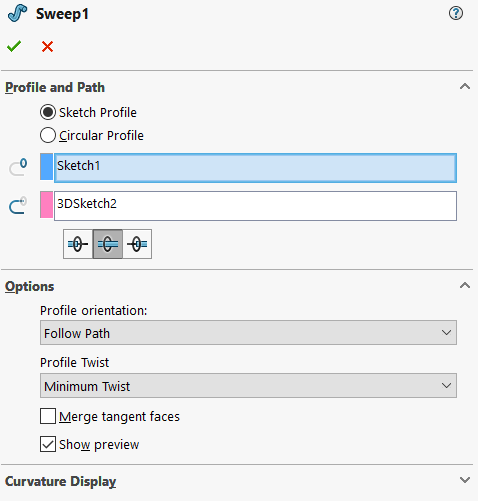
\includegraphics[height=4in]{images/figures/sweep-feature-tree.png}
\end{center}
\caption{Sweep property manager dialog. \label{fig:sweep-feature-tree}}

\end{figure}

\begin{figure}[H]
\begin{center}
  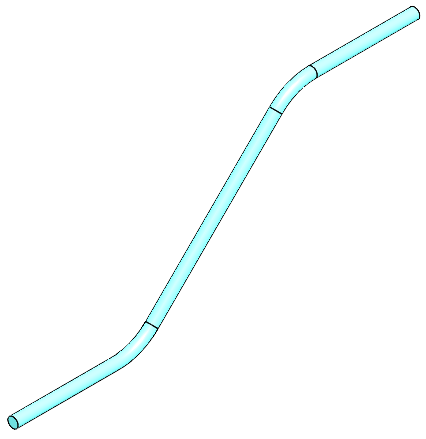
\includegraphics[height=3in]{images/figures/completed-cable-sweep.png}
\end{center}
\caption{Completed cable sweep.
\label{fig:completed-cable-sweep}}

\end{figure}

\subsubsection{Section Recap}

\begin{enumerate}
\item{} Sketch a circular profile normal to the cable path. Dimension this circle to
0.1''.
\item{} Make a \relation{Sweep} using the cross section and path we've created. My settings are
shown in Figure \ref{fig:sweep-feature-tree}.
\item{} Save early and save often.
\end{enumerate}

\section{Make a (Half) Pulley with a Revolve}

\label{sec:make_the_pulley}

First, create a new \relation{Sketch} on the Front Plane, the same plane as our cable
cross-section. \relation{Show} the cable cross-section sketch (which was absorbed by our \kode{Sweep} feature), and use \kode{Convert Entities} 
\includegraphics{images/symbols/convert-entities.png}
to bring that circle to the current sketch. Select the newly-made circle and
select ``For construction''.

Next, make a pulley cross-section. My sketch is shown in Figure~\ref{fig:pulley-cross-section}. Close this sketch once its fully defined.

\begin{figure}[H]
\begin{center}
  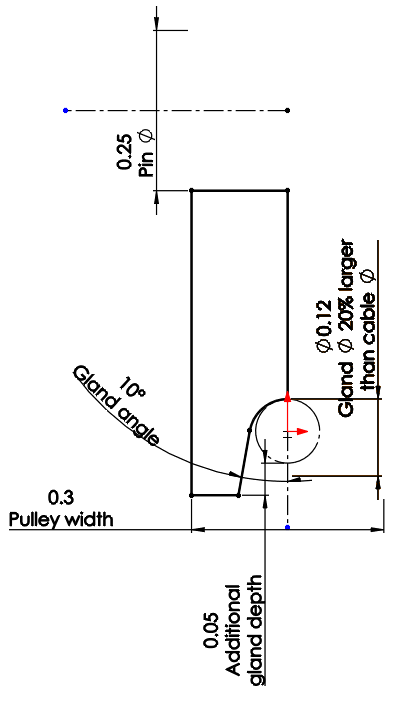
\includegraphics[height=4in]{images/figures/pulley-cross-section.png}
\end{center}
\caption{Pulley cross-section.
\label{fig:pulley-cross-section}}

\end{figure}

I won't talk through each aspect of the pulley, but I'll call out some features
that I feel are important.

\begin{itemize}
\item{} I explicitely CAD the rotational axis as a construction line in the sketch.
  This will provide my axis for the Revolve feature.
\item{} This rotational axis must be coincident with the center of \emph{Circle
  1}.
\item{} To add a dimension to the perimeter of a circle (rather than the
  center),
  hold \texttt{Shift} while clicking the circle. You can dimension the distance
  separating to circles' perimeters in the same fashion.
\item{} The gland of the pulley, where the cables ride, must be tangential to the
  cable cross-section, as shown in Figure \ref{fig:pulley-gland}, otherwise
  the cable won't ride where we want it to.
\item{} The gland diameter must be larger than the cable. Otherwise, the cable will get sucked into the pulley and will not roll smoothly. In this instance, I've made the gland diameter 20\% larger than the cable.
\item{} You can display the gland diameter as a diameter (rather than a radius)
  by right-clicking on the dimension and selecting "Display as Diameter".
\item{} The pulley gland should have a V-shaped entrance. This will reduce
cable-pulley interference when we add fleet angle in Section~\ref{sec:non-tangential-pulleys}. In this case, I've added 10\textdegree \ of clearance from center line.
\item{} I tend to only CAD one side of the pulley. First, its less features for me to
  define. Second, it will allow me to \kode{Move/Copy}\cadsymbol{move-copy} the part more easily.
\end{itemize}

\begin{figure}[H]
\begin{center}
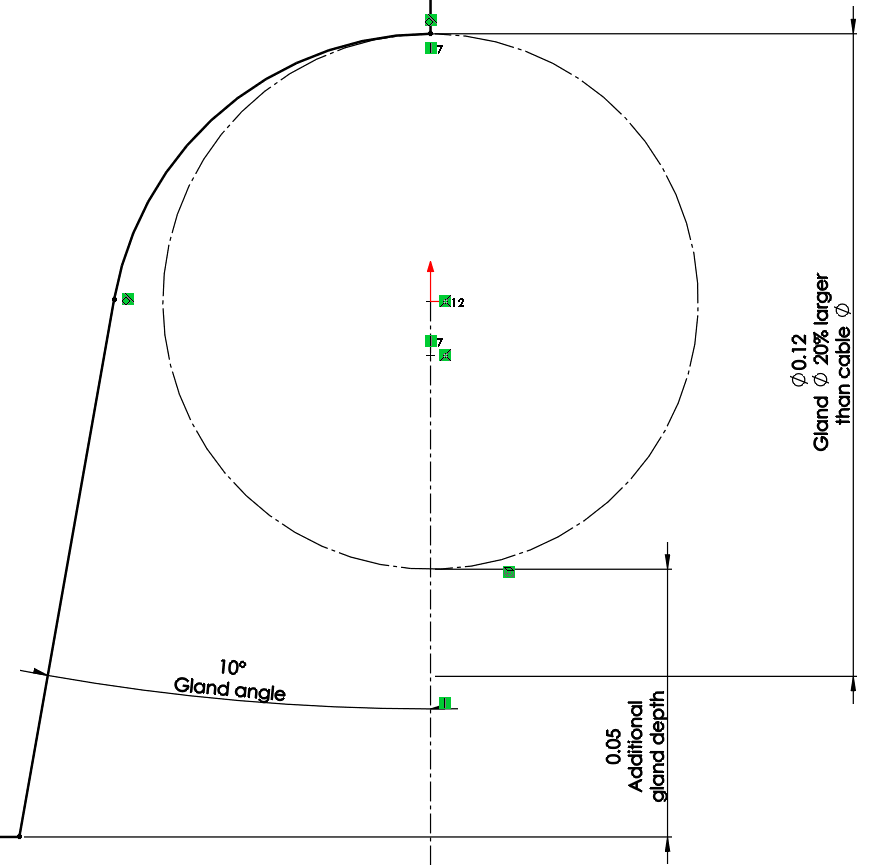
\includegraphics[height=4in]{images/figures/pulley-gland-details.png}
\end{center}
\caption{Pulley gland details. \label{fig:pulley-gland}}

\end{figure}

Finally, \relation{Revolve} the pulley profile about the construction line you added to
this sketch. Deselect ``Merge results''. If our pulleys and cables merge in real
life, something has gone very wrong. Close the feature

\includegraphics{images/symbols/green-check.png}. You should end up with half of a pulley, as
in Figure~\ref{fig:pulley-1-revolve}.

\begin{figure}[H]
\begin{center}
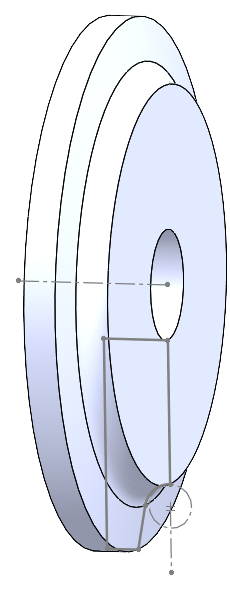
\includegraphics[height=3in]{images/figures/pulley-1-revolve.png}
\end{center}
\caption{Half of \emph{Pulley 1}, made with a \kode{Revolve}. Cable hidden for clarity.
\label{fig:pulley-1-revolve}}

\end{figure}

\subsubsection{Section Recap}

\begin{enumerate}
\item{} Create a pulley cross-section, as shown in Figure~\ref{fig:pulley-cross-section}.
\item{} \relation{Revolve} that cross-section about the pulley's central axis, arriving at
Figure~\ref{fig:pulley-1-revolve}.
\end{enumerate}

\section{Copy the Pulley to make Two}

\label{sec:copy_the_pulley}

\emph{Disclaimer: Depending on the part, I likely skip this step because I rarely
need both pulleys in the part file. Instead, I would duplicate the pulley in a
later assembly. I walk through it here because this tutorial is
accomplished in the Part file, not an Assembly file. I also walk through it here
because the Move/Copy feature is clunky to learn.}

\hfill\break

The next step to completing our assembly (which is a Part file containing
multiple solid bodies, not an assembly) is to copy our first pulley and move the copy to the
location of Circle 2. We will use the \kode{Move/Copy}\cadsymbol{move-copy} feature found under
\emph{Insert\textgreater{}Feature\textgreater{}Move/Copy}.

One infuriating fact of the Move/Copy feature is that if
you want to move a body using constraints (which we do), you cannot also make a
copy of it. You must add a separate feature to copy it. The dialog box for this
feature is shown in Figure~\ref{fig:copy-pulley-1}.

\begin{figure}[H]
\begin{center}
  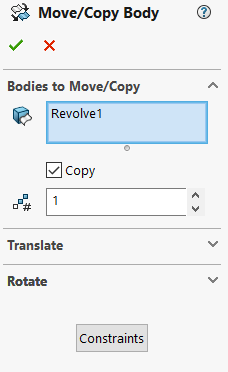
\includegraphics[height=2.5in]{images/figures/copy-pulley-1.png}
\end{center}
\caption{Move/Copy property manager for making a copy of Pulley 1.
\label{fig:copy-pulley-1}}

\end{figure}

Next, add a second \kode{Move/Copy}\cadsymbol{move-copy} feature with the dialog box shown in Figure~\ref{fig:move-pulley-1}. We'll add the following constraints to move the pulley to our desired location:

\begin{center}
\begin{tabular}{ccc}
\hline
  \relation{Coincident} & \emph{Circle 2} &
  \emph{Pulley 1 midplane face} \\
  \relation{Concentric} & \emph{Circle 2} &
  \emph{Pulley 1 midplane edge} \\
  \hline
\end{tabular}
\end{center}

\hfill\break

\begin{figure}[H]
\begin{center}
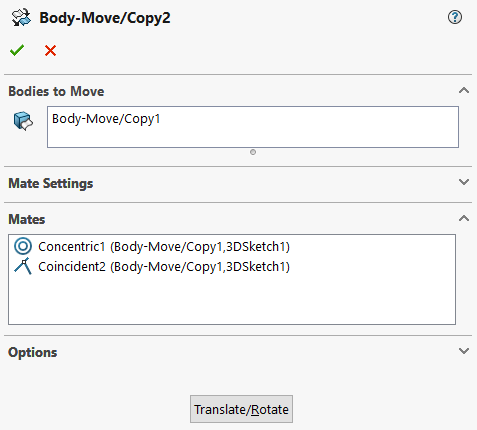
\includegraphics[height=4in]{images/figures/move-pulley-1.png}
\end{center}
\caption{Move/Copy property manager for moving Pulley 1 to the location of Pulley 2.
\label{fig:move-pulley-1}}

\end{figure}

We should now have a cable and two half-pulleys, as in
Figure~\ref{fig:cable-and-half-pulleys}.

\begin{figure}[H]
\begin{center}
  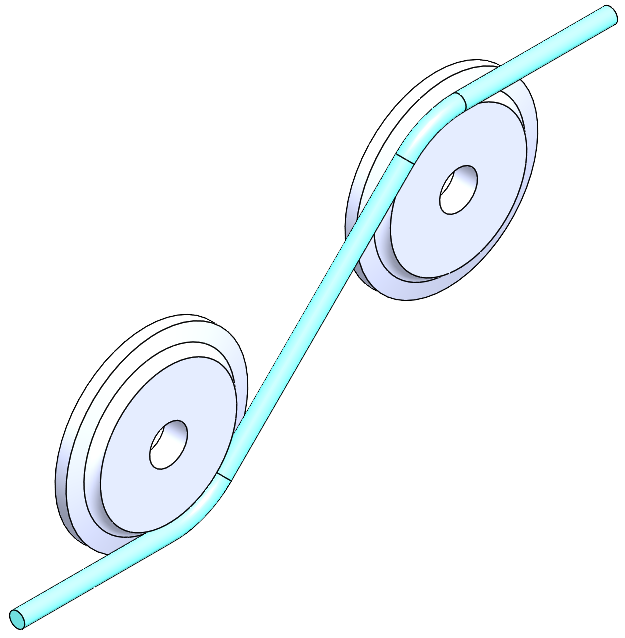
\includegraphics[width=3in]{images/figures/cable-and-half-pulleys.png}
\end{center}
\caption{Cable and two half-pulleys, after a pair of \kode{Move/Copy} features.
\label{fig:cable-and-half-pulleys}}

\end{figure}

\subsubsection{Section Recap}

\begin{enumerate}
\item{} Create a \kode{Move/Copy}\cadsymbol{move-copy} feature to duplicate Pulley 1, as shown in
Figure~\ref{fig:copy-pulley-1}.
\item{} Create a second \kode{Move/Copy}\cadsymbol{move-copy} feature to move Pulley 1 to the location of
Circle 2, as shown in Figure~\ref{fig:move-pulley-1}.
\end{enumerate}

\section{Making the Pulleys Whole}

\label{sec:mirror_pulleys}

Our final step is to make the pulleys whole. Add a \relation{Mirror} feature
to mirror Pulley 1 about its mid-plane. Be sure to use ``Bodies to Mirror''. Select ``Merge solids''. My
\kode{Mirror} dialog box is shown in Figure~\ref{fig:mirror-dialog}. Repeat this for
Pulley 2. It is important to create these mirrors as two separate features
because, later, the pulleys won't be in the same plane.

\begin{figure}[H]
\begin{center}
  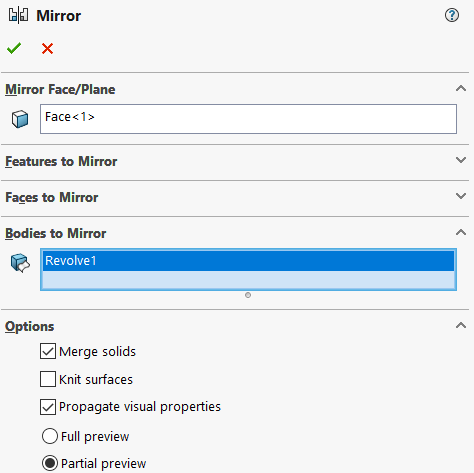
\includegraphics[height=4in]{images/figures/mirror-dialog.png}
\end{center}
\caption{Property manager for \kode{Mirror} of the pulley bodies. \label{fig:mirror-dialog}}

\end{figure}

Congratulations! We now have two pulleys and one cable
(Figure~\ref{fig:completed-planar2}), and if all went
smoothly, the cable will be tangential to both pulleys.

\begin{figure}[H]
\begin{center}
  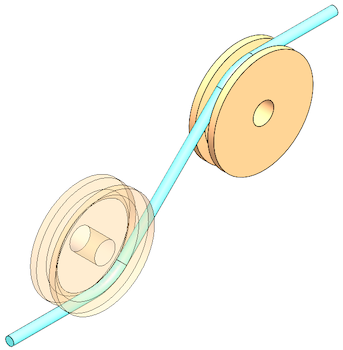
\includegraphics[width=3in]{images/figures/completed-planar.png}
\end{center}
\caption{Completed cable-pulley system with all components in one plane. One pulley is
transparent for clarity.
\label{fig:completed-planar2}}

\end{figure}

\subsubsection{Section Recap}

\begin{enumerate}
\item{} \relation{Mirror} \emph{Pulley 1} body to make a complete pulley.
\item{} \kode{Mirror} \emph{Pulley 2} body to make a complete pulley.
\item{} Save and celebrate.
\end{enumerate}

\begin{aside}
\label{box:keyboard_shortcuts}
\heading{Speeding Things Up}

All the best cadders I know move their mouse as little as possible. This is
because mouses require precision, and precision requires both time and skill.
But we can move faster without either of these things. Some designers prefer
mouse gestures, but I've never found them intuitive. I use keyboard shortcuts. I present my style here, but there's no need for you to adopt it. Styles aren't
right or wrong, but some are more useful than others.

My hotkeys are either chosen based on a mneumonic device (which I say in my head
as I type it), or they are based on Onshape's immutable hotkey choices. Of the features we'll use in this tutorial, here are the keyboard shortcuts I use.

\begin{tabular}{lcc}
                                    && \\
``When I need to use this feature'' & ``I use this hotkey'' & ``Which stands for:'' \\
  \hline
                                    && \\
\relation{Sketch} & \texttt{Shift+S} & From Onshape \\
\relation{Line} & \texttt{L} & ``Line'' \\
\relation{Centerline} & \texttt{Q} & From Onshape \\
\relation{Circle} & \texttt{C} & ``Circle'' \\
\relation{Trim} & \texttt{X} & ``X-Acto Knife'' \\
\relation{Dimension} & \texttt{D} & ``Dimension'' \\
\relation{Revolve} & \texttt{Ctrl+R} & ``Revolve'' \\
\relation{Mirror} & \texttt{Ctrl+M} & ``Mirror'' \\
\relation{Convert Entities} & \texttt{U} & ``Use'' \\
\relation{Hide All Types} & \texttt{Shift+R} & ``Show relations'' \\
\relation{Show Sketch Dimensions} & \texttt{Shift+D} & ``Show dimensions'' \\
\relation{Show Sketch Relations} & \texttt{Shift+R} & ``Show relations'' \\
\relation{Triad} & \texttt{T} & ``Triad'' \\
\relation{Section View} & \texttt{Alt+S} & ``Alternate section'' \\
\relation{Normal View} & \texttt{N} & ``Normal'' \\
\kode{Customize shortcuts} & \texttt{Alt+Shift+C} & ``Meta short cut'' \\

\end{tabular}

\end{aside}
